\documentclass[a4paper]{report}

\usepackage{../mathstemplate}

\date{IV семестр, весна 2024 г.}
\title{Математический анализ. Неофициальный конспект}
\author{Лектор: Сергей Витальевич Кисляков \\ Конспектировал Леонид Данилевич}

\begin{document}
    \shorthandoff{"}
    \maketitle
    \tableofcontents
    \newpage
    \setcounter{lection}{0}
    \chapter{Комплексный анализ}
    \newlection{16 февраля 2024 г.}
    Пусть $f: G \map \C$, где открытое $G \subset \C$.
    \definition[$f$ голоморфна в $z_0 \in G$]{
    $\exists \lim\limits_{z \to z_0}\frac{f(z) - f(z_0)}{z - z_0} \bydef f'(z_0)$.
    }
    Во втором семестре мы проверяли, что $f = u + iv$ (где $u, v: G \map \R$) голоморфна в $z_0 \iff f$ дифференцируема в вещественном смысле, и выполняются уравнения Коши --- Римана:
    \[\der{u}{x} = \der{v}{y} \qquad \der{u}{y} = -\der{v}{x}\]
    \definition[$f$ аналитична в $G$] {
    $\forall z_0 \in G: \exists c_j \in \C$: \[f(z) = \sum\limits_{j = 0}^{\infty}c_j(z - z_0)^j\tag{$*$}\label{analytic}\] где ряд сходится не только при $z = z_0$.
    }
    \theorem{\label{analytic-is-holomorphic}
    $f$ аналитична в $G \iff f$ голоморфна во всех точках $G$.
    \provetwhen{
        Доказали во втором семестре, несложно.
    }{
        Скоро займёмся, время пришло.
    }
    }
    Из представления~(\ref{analytic}) следует, что производная в точке $z$ считается почленно: $f'(z) = \sum\limits_{j = 1}^{\infty}j c_j (z - z_0)^{j - 1}$.
    В частности, отсюда получается, что $f'(z_0) = c_1$, и вообще $f^{(n)}(z_0) = j! \cdot c_j$.

    Вскоре мы увидим, что ситуация разительно отличается от вещественной: в вещественном случае были разные классы --- дифференцируемые функции, $C^1$, $C^\infty$, аналитичные, и множество промежуточных классов.

    В комплексном же случае, если функция хотя бы один раз дифференцируема, то окажется, что этого достаточно, чтобы она была не просто дифференцируема, а непрерывно дифференцируема, бесконечно дифференцируема, и даже аналитична.
    \section{Интеграл от дифференциальной формы вдоль пути}
    \subsection{Про дифференциальные формы}
    \definition[Линейная функция $l: \R^n \map \C$]{${\forall \alpha, \beta \in \R, x, y \in \R^n: l(\alpha x + \beta y) = \alpha l(x) + \beta l(y)}$.}
    \definition[Линейная форма на множестве $G \subset \R^n$]{
    Функция двух переменных ${\phi: G \times \R^n \map \C}$, линейная по второму аргументу.
    }
    В пространстве $\R^n$ имеется базис $(e_j)$: $h = e_1 h_1 + \dots + e_n h_n$.

    Тем самым, $\phi(x, h) = \sum\limits_{j = 1}^{n}\underbrace{\phi(x, e_j)}_{\eqqcolon g_j(x)}h_j = \sum\limits_{j = 1}^{n}g_j(x)h_j$.

    Введём \emph{базисные линейные формы} $\d x_j(u, h) = h_j$, игнорирующую первую координату, и возвращающая $j$-ю компоненту второго аргумента.
    Теперь $\phi(x, h)$ разложилась в сумму $\sum\limits_{j = 1}^{n}g_j \d x_j$.

    \example{
        Пусть $f: G \map \C$ --- дифференцируемая в $G$ функция.
        Заметим, что её дифференциал $\d_f(x, \_)$ --- в точности линейная форма на $G$.

        При разложении по базису получится $\d_f(x, \_) = \sum\limits_{j = 1}^{n}\der{f}{x_j}(x)\d x_j$.
    }
    Вскоре мы увидим, что далеко не всякая линейная форма является чьим-то дифференциалом.

    Если $\phi = \sum\limits_{j = 1}^{n} g_j\d x_j$ --- дифференциал функции $f$, то непременно $g_j = \der{f}{x_j}$.

    Тот факт, что $\phi$ является дифференциалом $f$, можно сказать наоборот: $f$ является первообразной $\phi$.
    \subsection{Про интегрирование}
    Рассмотрим монотонную функцию $\Phi: \angles{a, b} \map \R$.
    Как и при определении стилтьесовой длины, будем считать, что $\Phi$ определена на некотором открытом множестве, содержащем $\angles{a, b}$.
    Обозначим за $l_\Phi$ стилтьесову длину, отвечающую функции $\Phi$.

     Пускай $\lambda_\Phi$ --- продолжение стилтьесовой длины $l_\Phi$ по Лебегу --- Каратеодори.

    Она, как водится, определена на некоторой $\Sigma$-алгебре, в которой есть борелевские множества, но измеримы могут быть и какие-то другие множества, зависящие от конкретной функции $\Phi$.
    \examples{
        \item Так, функция $\phi(x) = \all{0,&x < 0 \\ 1,& x \ge 0}$ порождает дельта-меру $\delta_0$, относительно которой все множества измеримы.

        Кроме того, эта мера сингулярна относительно стандартной меры Лебега.

    \item Может показаться, что так происходит из-за разрывности $\phi$, но это не так.

        Рекурсивно определим канторову лестницу $C: [0, 1] \map [0, 1]$:
        \[\begin{tikzpicture}[scale=1]
              \draw[->] (-0.5,0) -- (3.5,0) node[above]{$x$};
              \draw[->] (0,-0.5) -- (0,3.5) node[right]{$y$};
              \fill (0, 0) circle (1.5pt) node[below left] {$0$};
              \fill (1, 0) circle (1.5pt) node[below] {$\nicefrac13$};
              \fill (2, 0) circle (1.5pt) node[below] {$\nicefrac23$};
              \fill (3, 0) circle (1.5pt) node[below] {$1$};
              \fill (0,1.5) circle (1.5pt) node[left] {$\nicefrac12$};
              \fill (0,3) circle (1.5pt) node[left] {$1$};
              \newcommand{\cantor}[5]{ %l, r, d, u, depth
                  \pgfmathsetmacro{\depth}{\numexpr#5}

                  \draw ({(#1+2*#2)/3},{(#3+#4)/2}) -- ({(2*#1+#2)/3},{(#3+#4)/2});

                  \ifnum\depth<5
                  \cantor{#1}{(2*#1+#2)/3}{#3}{(#3+#4)/2}{#5+1}
                  \cantor{(#1+2*#2)/3}{#2}{(#3+#4)/2}{#4}{#5+1}
                  \else
                  \draw ({#1}, {#3}) -- ({#2}, {#4});
                  \fi
              }
              \cantor{0}{3}{0}{3}{0}
        \end{tikzpicture}\]
        Построив по данной функции стилтьесову длину $\lambda_C$, мы получим меру, сосредоточенную на канторовом множестве меры нуль.

        Её носитель --- само канторово множество, так как на всех отрезках вне канторова множества $\lambda_C$ равна нулю.
        Она сингулярна относительно стандартной меры Лебега на $\R$, и её измеримые множества разительно отличаются от измеримых множеств меры Лебега.
    }
    По мере Стилтьеса можно интегрировать: если $v$ является $\lambda_\Phi$ измеримой (в частности, измерима по Борелю и непрерывна), то определён интеграл $\int\limits_{\angles{a, b}}v \d\lambda_{\Phi}$
    Иногда пишут просто $\int\limits_{\angles{a, b}}v \d \Phi$. %Так складывается ощущение, что из измеримости следуют и борелевская измеримость, и непрерывность. % ок, заменю "и даже" на "и"
    \ok
    Теперь пусть $I = [a, b]$, и $\Psi: [a, b] \map \R$ --- функция ограниченной вариации.
    В таком случае $\Psi = \Phi_1 - \Phi_2$, где некие $\Phi_1, \Phi_2$ возрастают.
    Можно определить знакопеременную меру $\lambda_\Psi \bydef \lambda_{\Phi_1} - \lambda_{\Phi_2}$, понятно, что определение корректно.
    \subsection{Интеграл от дифференциальной формы вдоль пути}
    Пускай $\gamma: [a, b] \map G \subset \R^n$ --- спрямляемый путь (путь конечной длины).
    Пускай $U = \sum\limits_{j = 1}^{n}u_j \d x_j$ --- дифференциальная форма в области $G$.
    Если не сказано противное, будем считать, что $u_j$ --- непрерывные функции.
    \definition[Интеграл от $U$ вдоль пути $\gamma$]{
    $\int\limits_{\gamma}U \bydef \sum\limits_{j = 1}^{n}\int\limits_{[a, b]}u_j(\gamma(t))\d \gamma_j(t)$.
    }
    Здесь $\gamma = (\gamma_1, \dots, \gamma_n)$.
    Так как путь спрямляем, то все $\gamma_j$ --- ограниченной вариации, каждая порождает свою меру Стилтьеса, и определение интегрирует композицию $U \circ \gamma$ по данной мере.
    \subsection{Сумма путей}
    Пускай имеются два отрезка $[a, c]$ и $[c, d]$, и на них заданы пути $\gamma_1: [a, c] \map G$, $\gamma_2: [c, d] \map G$.
    Предположим, что $\gamma_1(c) = \gamma_2(c)$.

    Тогда можно устроить путь $\gamma = \gamma_1 \oplus \gamma_2: [a, d] \map G$, $\gamma(t) \bydef \all{\gamma_1(t),&t \in [a, c] \\ \gamma_2(t),& t \in [c, d]}$.

    \note{
    Интеграл аддитивен по множеству: $\int\limits_{\gamma_1 \oplus \gamma_2}U = \int\limits_{\gamma_1}U + \int\limits_{\gamma_2}U$. %Мб тут вставить ", поэтому", а тто так не выглядит, как по множеству.
    }
    \subsection{Альтернативное определение}
    Далее мы не интересуемся никакими чудесами вроде канторовых лестниц, и считаем, что $\Phi$ такова, что $\lambda_\Phi$ абсолютно непрерывна относительно стандартной меры Лебега.

    А раз так, то по теореме Радона --- Никодима $\exists$ суммируемая $w: [a, b] \map \R$, такая, что \[\lambda_\Phi(e) = \int\limits_{e}w(x)\d x\tag{$+$}\label{density}\]
    \fact{\label{density-is-derivative}
        Формула~(\ref{density}) заведомо верна, если $\Phi$ непрерывно дифференцируема на $[a, b]$, тогда $w = \Phi'$.
        \provehere{
            Введём меру $\nu(e) = \int\limits_{e}\Phi'(x)\d x$, заданную на измеримых по Лебегу множествах.
            $\Phi'$ непрерывна, и, следовательно, измерима.

            Если $\angles{c, d} \subset [a, b]$, то $\nu(\angles{c, d}) = \int\limits_{\angles{c, d}}\Phi'(x)\d x = \Phi(d) - \Phi(c) = l_\Phi(\angles{c, d})$.

            Таким образом, из теоремы единственности, продолжение $l_\Phi$ по Лебегу --- Каратеодори совпадает с $\int\limits_{e}\Phi'(x)\d x$.
        }
    }
    \note{
        Утверждение~(\cref{density-is-derivative}) сохраняет силу, если $\Phi$ непрерывна и кусочно-непрерывно дифференцируема.
    }
    \comment{Далее где-то используется $\Phi$, а где-то $\beta$, надо убедиться, что это везде одно и то же, и заменить. } % тогда и я трогать эти две буквы пока не буду
    Пускай $\beta: [a, b] \map \R$ --- функция ограниченной вариации, кусочно-непрерывно дифференцируемая: $\exists a = a_0 < a_1 < \dots < a_k = b$, такие, что $\beta$ непрерывно дифференцируема на $[a_s, a_{s+1}]$ при $0 \le s < k$.
    Введём $\rho(e) = \int\limits_{e}\beta'(x)\d x$ --- это знакопеременная вещественная мера.

    У данной меры возникают (см. разложение Хана) положительная и отрицательная части $\rho_+(e) \bydef \int\limits_{e}(\beta')_+(x)\d x$ и $\rho_-(e) \bydef \int\limits_{e}(\beta')_-(x)\d x$
    
    Если обозначить за $\Phi_+(t) = \int\limits_{0}^{t}(\beta')_+(x)\d x$ и $\Phi_-(t) = \int\limits_{0}^{t}(\beta')_-(x)\d x$, то окажется, что соответствующие меры Стилтьеса совпадают с $\rho_+$ и $\rho_-$.
    
    Более того, $\beta = \Phi_+ - \Phi_-$ --- получили разложение функции ограниченной вариации в положительную и отрицательную части.
    \note{
    Это разложение экономнее, чем то, которое было получено ранее --- ранее в качестве $\Phi_+$ выбиралась вариация $\Phi$.
    }
    
    Если всё, что написано выше, собрать вместе, то получится 
    \encircle{\int\limits_{[s, t]}v \d \Phi = \int\limits_{[s, t]}v(x)\beta'(x)\d x}
    Далее <<гладкий>> используется, как синоним к непрерывно-дифференцируемому.
    \corollary[Можно считать определением]{
        Если $U = \sum\limits_{j = 1}^{n}u_j \d x_j$ --- дифференциальная форма в $G$ с непрерывными коэффициентами, а $\gamma = (\gamma_1, \dots, \gamma_n): [a, b] \map G$ --- спрямляемый кусочно-гладкий путь, то
    \[\int\limits_{\gamma}U = \sum\limits_{j = 1}^{n}\int\limits_{a}^{b}u_j(\gamma(t))\gamma_j'(t)\d t\]
    }
    \subsection{(Не)зависимость от параметризации}
    Пускай $\gamma: [a, b] \map G$ --- кусочно-гладкий путь, $\psi: [c, d] \map [a, b]$ --- гладкий гомеоморфизм.

    Теперь $\tilde{\gamma} = \gamma \circ \psi$ --- перепараметризация $\gamma$
    \lemma{
        Для всякой формы $U$:
        \[\int\limits_{\tilde{\gamma}}U = \pm\int\limits_{\gamma}U\]
        Знак $+$ выбирается, если $\psi$ возрастает, и $-$ --- если убывает.
        \provehere{
            Предположим, что $\gamma$ --- гладкий путь, иначе применяем к кусочкам гладкости по отдельности.

            $\int\limits_{\tilde{\gamma}}U = \sum\limits_{j = 1}^{n}\int\limits_{c}^{d}u_j(\gamma(\psi(t)))\gamma_j'(\psi(t))\cdot \psi'(t)\d t = \left\|\arr{c}{\tau = \psi(t) \\ \d \tau = \psi'(t)\d t}\right\| = \sum\limits_{j = 1}^{n}\int\limits_{\psi(c)}^{\psi(d)}u_j(\gamma(\tau))\gamma_j'(\tau)\d \tau = \pm \int\limits_{\gamma}U$
        }
    }
    Про $\psi$ также можно считать, что это он не гладкий, а лишь кусочно-гладкий.

    Тем самым, можно определить сумму путей для несоприкасающихся отрезков: для двух путей $\gamma_1: [a, b] \map G, \gamma_2: [c, d] \map G$ (при условии $\gamma_{1}(b) = \gamma_2(c)$) можно один их отрезков-прообразов линейным возрастающим преобразованием перевести в отрезок, соприкасающийся со вторым (например, $t \mapsto t + (b - c)$).

    Также есть понятие обратного пути $\gamma^-(t) = \gamma(a + b - t)$.
    Для любой формы $U$: \[\int\limits_{\gamma \oplus \gamma^-}U = \int\limits_{\gamma}U + \int\limits_{\gamma^-}U = \int\limits_{\gamma}U - \int\limits_{\gamma}U = 0\]
    \section{Условия существования первообразной у дифференциальной формы}
    \theorem{
    Если у дифференциальной формы $U$ в открытом множестве $G \subset \R^n$ имеется первообразная $F$, то для всякого кусочно-гладкого пути $\gamma: [a, b] \map G$
    \[\int\limits_{\gamma}U = F(\gamma(b)) - F(\gamma(a))\]
    \provehere{
        $U = \sum\limits_{j = 1}^{n}g_j \d x_j$, где $g_j(w) = \der{}{x_j}F(w)$.
        Считаем, что путь гладкий.
    \[\int\limits_{\gamma}U = \sum\limits_{j = 1}^{n}\int\limits_{a}^{b}\der{}{x_j}F(\gamma(t))\gamma_j'(t)\d t = \int\limits_{a}^{b}\frac{\d}{\d t}(F \circ \gamma)(t)\d t = F(\gamma(b)) - F(\gamma(a))\]
    Если же путь всего лишь кусочно-гладкий, то надо разбить отрезок на подотрезки гладкости, и сложить.
    }
    }
    \corollary{
    Если у дифференциальной формы $U$ есть первообразная, то её интегралы по всем путям с данными началом и концом, равны.
    }
    Оказывается, верно и обратное.
   %Надо пересмотреть написание "кусочно-непрерывно дифференцируемый", я нашёл вариант с двумя дефисами.
    \newlection{26 февраля 2024 г.}
    \lemma{
        Пусть $G$ --- область в $\R^n$, тогда любые две её точки можно соединить ломаной (кусочно-линейным путём).
    \provehere{
        Выберем $x_0 \in G$, положим $U = \defset{y \in G}{\text{существует ломаная в $G$ с началом в $x_0$ и концом в $y$}}$.

        Покажем, что $U$ открыто.
        Пусть $y \in U$, тогда найдётся шарик $B_\eps(y) \subset G$, и $B_\eps(y) \subset U$ --- можно добавить одно звено к ломаной $x_0 \rightsquigarrow y$.

        Покажем, что $U$ замкнуто.
        Пусть $z \in G$ --- предельная точка для $U$. Найдётся $B_\eps(z) \subset G$, так как $z$ --- предельная, то $\exists y \in B_\eps(z) \cap U$.
        Значит, $z \in U$ --- можно добавить одно звено $y \rightarrow z$.
    }
    }
    \note{
        Имея кусочно-линейный путь $\gamma: [a, b] \map G$, соединяющий $A,B \in G$, несложно получить бесконечно дифференцируемый путь, соединяющий их:

        Пусть $\gamma_1: [a - 1, b + 1] \map G, \gamma_1(t) = \all{\gamma(t),&t \in [a, b] \\ \gamma(a),& t \in [a-1, a] \\ \gamma(b),&t \in [b, b + 1]}$.
        Теперь, сворачивая $\gamma_1$ с аппроксимативной единицей с достаточно большим номером и достаточно малым компактным носителем, получим бесконечно дифференцируемый путь, соединяющий $A$ и $B$.
    }
    \theorem{\label{integral-along-path}
        Пусть $\Phi = \sum\limits_{j = 1}^{n}f_j(x)\d x_j$ --- \emph{непрерывная} дифференциальная форма в $G$ (то есть коэффициенты непрерывны в $G$).
        Следующие условия эквивалентны.
        \numbers{
        \item У $\Phi$ есть первообразная $F$, то есть функция $F \in C^1(G): \d F = \Phi$ (иными словами, $\forall j: \der{}{x_j}F = f_j$).
        \item Для всех кусочно-гладких путей $\gamma$ с фиксированными началом и концом $\gamma(a) = \gamma_a, \gamma(b) = \gamma_b$: $\int\limits_{\gamma}\Phi$ не зависит от $\gamma$ (а только от начала и конца).
        \item Для любой кусочно-гладкой петли (то есть замкнутого пути) $\gamma$ в $G$:  $\int\limits_{\gamma}\Phi = 0$.
        }
%        такова, что $\forall x, y \in G: \exists c \in \C: \forall$ кусочно-гладкого пути $\gamma$ с началом в $x$ и концом в $y$: $\int\limits_{\gamma}U = c$.
%        Эквивалентно, для всех замкнутых кусочно-гладких путей $\gamma: \int\limits_{\gamma}U = 0$.

%        Тогда $U$ обладает первообразной.
        \provehere{
            Мы уже доказали ранее цепочку импликаций $(1) \then (3) \then (2)$. Далее доказываем $(2) \then (1)$.

            Предъявим кандидат в первообразную.
            Зафиксируем $x_0 \in G$, выберем $x \in G$, пусть $\gamma$ --- произвольный кусочно-гладкий путь с началом в $x_0$ и концом в $x$.
            Определим $F(x) \bydef \int\limits_{\gamma}\Phi$.
            Согласно посылке, $F$ корректно определена --- не зависит от выбора пути.

            Покажем, что частные производные $F$ существуют, и равны $f_j$.
            Тогда они получатся непрерывными, то есть $F$ --- дифференцируемой, и окажется, что $F$ --- первообразная $\Phi$.

            Пусть $e_1, \dots, e_n$ --- стандартные базисные орты в $\R^n$.
            Рассмотрим $\frac{F(x + t e_j) - F(x)}{t}$.

            При малых $t$: отрезок между $x$ и $x + t e_j$ лежит внутри $G$.
            Пусть $\gamma_1$ --- путь, соединяющий $x_0$ и $x$, $l$ --- отрезок от $x$ до $x + t e_j$.
        \[\frac{F (x + te_j) - F(x)}{t} = \frac{1}{t}\left(\int\limits_{\gamma_1 \oplus l}\Phi - \int\limits_{\gamma_1}\Phi\right) = \frac{1}{t}\int\limits_{l}\Phi = \frac1t \int\limits_{0}^{t}f_j(x + \tau e_j)\d \tau \underset{t \to 0}\Map f_j(x)\qedhere\]
        }
    }
    \definition[Прямоугольник на плоскости]{
    Множество вида $[a, b] \times [c, d] \subset \R^2$.
    }
    Область $G$ на плоскости будем называть \emph{удобной}, если $\exists x_0 \in G: \forall y \in G: \exists$ прямоугольник $P \subset G$, содержащий точки $x$ и $y$.
    \examples[Удобные области]{
    \item $\Int Q$, если $Q$ --- прямоугольник. В качестве центра $x_0$ подойдёт любая точка.
    \item $B_r(x_0) = \defset{x \in \R^2}{|x - x_0| < r}$. В качестве центра $x_0$ стоит взять центр, иначе не получится:
    \[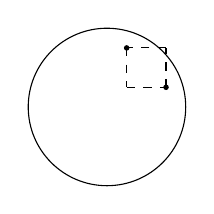
\begin{tikzpicture}
          \draw (0, 0) circle [radius=1];
          \fill (0.25,0.75) circle (1pt);
          \fill (0.75,0.25) circle (1pt);
          \draw[dashed] (0.25,0.75) -- (0.25, 0.25);
          \draw[dashed] (0.25,0.25) -- (0.75, 0.25);
          \draw[dashed] (0.75,0.25) -- (0.75, 0.75);
          \draw[dashed] (0.75,0.75) -- (0.25, 0.75);
    \end{tikzpicture}\]
    }
    \definition[Ориентированная граница прямоугольника $P$]{
    Петля $\gamma$, обходящая границу $P = [a, b] \times [c, d]$ против часовой стрелки, то есть вот так:
    \[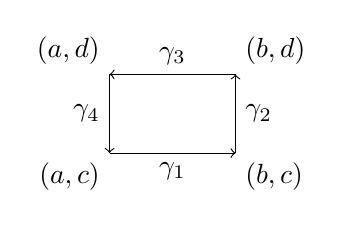
\begin{tikzpicture}
          \draw (0,0) node[below left] {$(a, c)$};
          \draw (0,1) node[above left] {$(a, d)$};
          \draw (1.6,0) node[below right] {$(b, c)$};
          \draw (1.6,1) node[above right] {$(b, d)$};

          \node at (0.8,0) [below] {$\gamma_1$};
          \node at (1.6,0.5) [right] {$\gamma_2$};
          \node at (0.8,1) [above] {$\gamma_3$};
          \node at (0,0.5) [left] {$\gamma_4$};

          \draw[->] (0,0) -- (1.6, 0);
          \draw[->] (1.6,0) -- (1.6, 1);
          \draw[->] (1.6,1) -- (0, 1);
          \draw[->] (0,1) -- (0, 0);
    \end{tikzpicture}\]
    $\gamma = \gamma_1 \oplus \gamma_2 \oplus \gamma_3 \oplus \gamma_4$.
    }
    Для прямоугольника $P$ будем обозначать за $\partial P$ в зависимости от контекста либо границу $P$, как топологического подмножества $\R^2$, либо путь, обходящий границу $P$ против часовой стрелки.
    \corollary[Дополнение к~(\cref{integral-along-path})]{
        Если $G$ --- удобная область на плоскости, то к трём эквивалентным условиям~(\cref{integral-along-path}) можно добавить
    \numbers{
    \item[4.] $\forall P \subset G: \int\limits_{\partial P}\Phi = 0$.
    }
    \provehere{
    $(3) \then (4)$ ясно, докажем $(4) \then (1)$.

    Пусть $x_0 \in G$ --- центр удобной области, определим $F(x) = \int\limits_{\delta}\Phi$, где $\delta$ --- это либо $\delta_1 \coloneqq \gamma_1 \oplus \gamma_2$ либо $\delta_2 \coloneqq \gamma_4^- \oplus \gamma_3^-$ (вне зависимости от выбора $\delta$ получится одно и то же).
        \[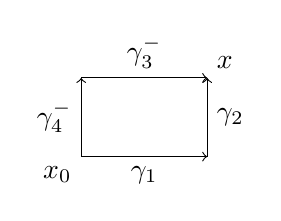
\begin{tikzpicture}
              \draw (0,0) node[below left] {$x_0$};
              \draw (1.6,1) node[above right] {$x$};

              \node at (0.8,0) [below] {$\gamma_1$};
              \node at (1.6,0.5) [right] {$\gamma_2$};
              \node at (0.8,1) [above] {$\gamma_3^-$};
              \node at (0,0.5) [left] {$\gamma_4^-$};

              \draw[->] (0,0) -- (1.6, 0);
              \draw[->] (1.6,0) -- (1.6, 1);
              \draw[<-] (1.6,1) -- (0, 1);
              \draw[<-] (0,1) -- (0, 0);
        \end{tikzpicture}\]
    Далее, чтобы проверить $\der{}{x_1}F = f_1$ и $\der{}{x_2}F = f_2$, воспользуемся подходящим представлением: пусть орт выглядит так: % "орт" --- это один, что тут имеется ввиду? "пусть орты расположены так"?
        \[\begin{tikzpicture}[scale=1]
            \draw[->](0,0) -- (0,1) node [below left] {$x_1$};
            \draw[->](0,0) -- (1,0) node [below left] {$x_2$};
        \end{tikzpicture}\]
        тогда для проверки $\der{}{x_1}F = f_1$ удобно воспользоваться определением $F$ через $\delta_1$, для проверки $\der{}{x_2}F = f_2$ --- определением через $\delta_2$. Далее повторяем рассуждение из (\cref{integral-along-path}).
    }
    }
    Пусть $\Phi = \sum\limits_{j = 1}^{n}f_j(x)\d x_j$ --- непрерывная дифференциальная форма в области $G \subset \R^n$.
    \definition[Форма $\Phi$ точна]{Существует первообразная $F$ в $G: \d F = \Phi$. }
    \definition[Форма $\Phi$ замкнута]{ Форма $\Phi$ локально точна ($\forall x_0 \in G: \exists U \ni x_0$: $\Phi\big|_U$ точна). }
    Понятно, что точная форма замкнута, но точность из замкнутости не следует: чуть позднее мы определим $\d z$, и покажем, что $\frac{\d z}{z}$ --- замкнутая, но не точная форма на $\C \sm \{0\}$
    \theorem{
    Пусть $\Phi$ --- дифференциальная форма в области $G \subset \R^n$.
        Следующие условия эквивалентны:
    \numbers{
    \item $\Phi$ замкнута.
    \item $\forall x_0 \in G: \exists V \ni x_0: \forall$ кусочно-гладкого замкнутого пути $\gamma$ с носителем в $V$: $\int\limits_{\gamma}\Phi = 0$.
    }
    Если $n = 2$, то дополнительно появляются ещё два условия:
    \numbers{
    \item[3.] $\forall z \in G: \exists \underset{\ni z}{V_z} \subset G: \forall P \subset V_z: \int\limits_{\partial P}\Phi = 0$.
    \item[4.] $\forall P \subset G: \int\limits_{\partial P}\Phi = 0$.
    }
    \provehere{
    Докажем, что $(3) \then (4)$, остальное уже доказано выше.

    Заметим, что границу прямоугольника $P$ можно представить, как сумму границ четырёх прямоугольников вдвое меньшего диаметра:
        \[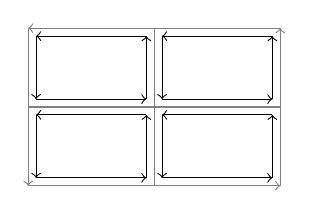
\begin{tikzpicture}
              \draw[->,color=gray] (0,0) -- (3.2, 0);
              \draw[->,color=gray] (3.2,0) -- (3.2, 2);
              \draw[->,color=gray] (3.2,2) -- (0, 2);
              \draw[->,color=gray] (0,2) -- (0, 0);
              \draw[color=gray] (0,1) -- (3.2,1);
              \draw[color=gray] (1.6,0) -- (1.6,2);
              \foreach \x/\y in {0/0,1.6/0,0/1,1.6/1} {
                  \draw[->] ({\x+0.1},{\y+0.1}) -- ({\x+1.5}, {\y+0.1});
                  \draw[->] ({\x+1.5},{\y+0.1}) -- ({\x+1.5}, {\y+0.9});
                  \draw[->] ({\x+1.5},{\y+0.9}) -- ({\x+0.1}, {\y+0.9});
                  \draw[->] ({\x+0.1},{\y+0.9}) -- ({\x+0.1}, {\y+0.1});
              }
        \end{tikzpicture}\]

    Таким образом, чтобы доказать, что интеграл по границе большого прямоугольника $P$ нулевой, разобьём его на достаточно маленькие прямоугольники, по ним-то интеграл нуль.
    Чтобы это формализовать, вспомним лемму Лебега о покрытии:
    \theorem[Лемма Лебега]{
    Пусть $K$ --- компакт в метрическом пространстве, $\{U_j\}_{j \in J}$ --- открытое покрытие компакта $K$. Тогда $\exists \delta > 0: \forall A \subset K: \diam A < \delta \then \exists j \in J: A \subset U_j$.
    }
    Применяя лемму Лебега для покрытия $P$ окрестностями $\{V_z\}_{z \in P}$, получим такое число $\delta$. Теперь надо разбить границу прямоугольника $P$ в сумму границ прямоугольников диаметра меньше $\delta$, а посылка теоремы говорит, что интеграл по ним уже нуль.
    }
    }
    \section{Операторы $\der{}{z}$ и $\der{}{\overline{z}}$}
    Как известно, $\C = \defset{x + iy}{x, y \in \R}$, то есть $\forall z \in \C: z = x + iy$, аналогично $\overline{z} = x - iy$.

    Рассмотрим $z$ и $\overline{z}$, как функции $\R^2 \map \C, (x, y) \mapsto x \pm iy$.
    Теперь $\d z = \d x + i \d y$ и $\d \overline{z} = \d x - i \d y$ образуют базис в пространстве дифференциальных форм (тех, которые не зависят от точки), обратное преобразование выглядит так:
    \[\all{\d x = \frac{\d z + \d \overline{z}}{2} \\ \d y = \frac{\d z - \d \overline{z}}{2i}}\]
    Рассмотрим форму $\Phi: \R^2 \map \C, \Phi(x, y) = \alpha(x, y)\d x + \beta(x, y)\d y$.
    Перепишем её в новом базисе:
    \[\Phi(x, y) = \frac{\alpha(x, y)}{2}(\d z + \d \overline{z}) + \frac{\beta(x, y)}{2i}(\d z - \d\overline{z}) = \frac{\alpha(x, y) - i \beta(x, y)}{2}\d z + \frac{\alpha(x, y) + i \beta(x, y)}{2}\d \overline{z}\]
    Теперь пусть $\Phi$ --- точная форма, то есть $\Phi = \d F$, и тогда $\alpha(x, y) = \der{}{x}F(x, y)$ и $\beta(x, y) = \der{}{y}F(x, y)$. Теперь
    \[\d F = \frac{1}{2}\left(\der{F}{x} - i\der{F}{y}\right)\d z + \frac{1}{2}\left(\der{F}{x} + i \der{F}{y}\right)\d \overline{z}\]
    \definition[$\der{F}{z}$]{
    Коэффициент, стоящий перед $\d z$, то есть $\frac{1}{2}\left(\der{F}{x} - i\der{F}{y}\right)$.
    }
    \definition[$\der{F}{\overline{z}}$]{
    Коэффициент, стоящий перед $\d \overline{z}$, то есть $\frac{1}{2}\left(\der{F}{x} + i \der{F}{y}\right)$.
    }
    Иначе говоря, мы ввели операторы $\der{}{z} \bydef \frac{1}{2}\left(\der{}{x} - i\der{}{y}\right)$ и $\der{}{\overline{z}} \bydef \frac{1}{2}\left(\der{}{x} + i \der{}{y}\right)$ так, что \[\d F = \der{}{z}F\d z + \der{}{\overline{z}}F\d\overline{z}\]
    \subsection{Связь с голоморфными функциями}
    Пусть $F = u + iv$, где $u, v: \R^2 \map \R$.
    Запишем
    \[\der{F}{\overline{z}} = \frac{1}{2}\left(\der{u}{x} + i\der{v}{x} + i\left(\der{u}{y} + i\der{v}{y}\right)\right) = \frac12\left(\left(\der{u}{x} - \der{v}{y}\right) + i\left(\der{v}{x} + \der{u}{y}\right)\right)\]
    В правой части равенства получились выражения из уравнений Коши --- Римана.
    \fact{
    Вещественные функции $u, v$ удовлетворяют уравнениям Коши --- Римана $\iff \der{(u + iv)}{\overline{z}} \equiv 0$.
    }
    \fact{
    $F$ голоморфна $\iff \d F = \der{F}{z}\d z$.
     При этом $\der{F}{z}$ есть производная $F$ по комплексному аргументу.
        \provehere{
            Функция дифференцируема по комплексному аргументу $\iff$ её дифференциал --- умножение на комплексное число.
        }
    }
    В основном нас будут интересовать дифференциальные формы вида $\phi(z)\d z$, где $\phi$ --- произвольная функция.

    Выясним, когда у формы $\phi(z)\d z = \phi(z)\d x + i\phi(z)\d y$ имеется первообразная, то есть функция $g: \der{g}{x} = \phi, \der{g}{y} = i\phi$.
    Заметим, что $\der{g}{z} = \frac{1}{2}(\phi - i(i\phi)) = \phi$ и $\der{g}{\overline{z}} = \frac{1}{2}(\phi + i(i\phi)) = 0$.
    \statement{
    Форма $\phi\d z$ имеет первообразную $g \iff g$ голоморфна, и $g' = \phi$.
    }
    \theorem[Коши]{
    Если $g: G \map \C$ --- голоморфная функция (область $G \subset \C$), то форма $g(z)\d z$ замкнута.
    \provehere{Потом.}
    }
    \counterexample[Глобально первообразной может не быть]{
        Пусть $G = \C \sm \{0\}, g: G \map \C, g: z \mapsto \frac{1}{z}$.

    По теореме Коши у $g$ имеется локальная первообразная --- комплексный логарифм --- но глобально определить не получится.
        Пусть $\Gamma = \partial \mathbb{T}$ --- комплексная окружность, ориентируем её против часовой стрелки, а именно, рассмотрим стандартный обход окружности $\alpha: [0, 2\pi] \map \C,\: \alpha: \phi \mapsto e^{i\phi}$.
    Теперь убедимся, что форма не точна:
    \[\int\limits_{\alpha}\phi = \int\limits_{\alpha}\frac{\d z}{z} = \int\limits_{0}^{2\pi}\frac{\left(e^{it}\right)'}{e^{it}}\d t =\int\limits_{0}^{2\pi}\d t = 2\pi i \ne 0\]
    }
    Для будущих применений также определим ориентированную против часовой стрелки границу $B_r(z_0)$, это путь $\beta(t) = z_0 + r e^{i t}$ для $t \in [0, 2\pi]$.

    \example{
    Пусть $z_0, w \in \C, r \in \R_{> 0}$, $|w - z_0| \ne r$, пусть путь $\gamma$ обходит границу $B_r(z_0)$ против часовой стрелки:
        \[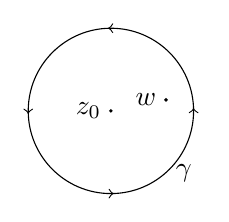
\begin{tikzpicture}[scale=0.7]
              \draw (0, 0) circle [radius=1.5];
              \fill (0, 0) circle (1pt) node[left] {$z_0$};
              \fill (1, 0.2) circle(1pt) node[left] {$w$};
              \draw[->] (1.5,-0.05) -- (1.5,0.05);
              \draw[->] (-1.5,0.05) -- (-1.5,-0.05);
              \draw[->] (0.05,1.5) -- (-0.05,1.5);
              \draw[->] (-0.05,-1.5) -- (0.05,-1.5);
              \node[below right] at (1,-0.8) {$\gamma$};
            \end{tikzpicture}\]
        Тогда, оказывается, (посчитаем чуть позже):
    \[\int\limits_{\gamma}\frac{\d z}{z - w} = \all{0,&|z - w| > r \\ 2\pi i,&|z - w| < r}\tag{$\circ$}\label{circle-integral}\]
    Грубой силой этот интеграл посчитать непросто, так как $w$ находится где угодно --- внутри или снаружи круга --- а интеграл, оказывается, зависит только от этих двух альтернатив.
    }
    \theorem[Основная оценка интеграла вдоль пути]{
        Пускай $\Phi = \sum\limits_{j=1}^n f_j\d x_j$ --- непрерывная дифференциальная форма в области $G \subset \R^n$, а $\gamma: [a, b] \map G$ --- кусочно-гладкий путь, $K \coloneqq \Image(\gamma) \subset G$.

    Тогда $\abs{\int\limits_{\gamma}\Phi} \le \underbrace{\sup\limits_{x \in K}\left(\sum\limits_{j = 1}^{n}|f_j(x)|^2\right)^{\nicefrac{1}{2}}}_{\eqqcolon A}\cdot l(\gamma)$.
    \provehere{
    Считаем, что $\gamma$ --- гладкий путь, иначе нужно разбить на кусочки гладкости.
    \[\abs{\int\limits_{\gamma}\Phi} = \abs{\int\limits_{a}^{b}\sum\limits_{j = 1}^{n}f_j\left(\gamma(t)\right)\gamma_j'(t)\d t} \underset{\text{КБШ}}\le \int\limits_{a}^{b}\left(\sum\limits_{j = 1}^{n}|f_j(\gamma(t))|^2\right)^{\nicefrac{1}{2}} \cdot \left(\sum\limits_{j = 1}^{n}|\gamma_j'(t)|^2\right)^{\nicefrac{1}{2}}\d t \le A \cdot \underbrace{\int\limits_{a}^{b}\left(\sum\limits_{j = 1}^{n}|\gamma_j'(t)|^2\right)^{\nicefrac{1}{2}}\d t}_{l(\gamma)}\]
    }
    }
    \newlection{1 марта 2024 г.}
    Рассмотрим дифференциальную форму $\Phi = F(z)\d z$, где $F$ --- непрерывная функция в $G \subset \C$.
    Пусть $\gamma: [a, b] \map G$ --- плоский путь.

    Расписав $\Phi(z) = F(z)\d x + i F(z)\d y$, и применяя основную оценку интеграла вдоль пути, получаем
    \[\abs{\int\limits_{\gamma}\Phi} \le \max\limits_{z \in K}\sqrt{|F(z)|^2 + |F(z)|^2} \cdot l(\gamma) = \sqrt{2}\max\limits_{z \in K}|F(z)| \cdot l(\gamma)\]
    Эта оценка вызывает некоторую неудовлетворённость: кажется, что $\sqrt{2}$ здесь лишний.
    И это действительно правда: можно расписать интеграл аккуратнее.

    Пусть $\gamma = \gamma_1 + i\gamma_2$, тогда по определению
    \[\int\limits_{\gamma}\Phi = \int\limits_{a}^{b}F(\gamma(t))\cdot \gamma_1'(t) + i F(\gamma(t))\cdot \gamma_2'(t)\d t = \int\limits_{a}^{b}F(\gamma(t)) \cdot \gamma'(t)\d t\]
    Таким образом, интеграл от комплексной формы вдоль пути имеет более простое представление, и оно легко поддаётся более плотной оценке:
    \[\abs{\int\limits_{\gamma}\Phi} \le \int\limits_{a}^{b}|F(\gamma(t))| \cdot |\gamma'(t)|\d t \le \max\limits_{z \in K}|F(z)| \underbrace{\int\limits_{a}^{b}|\gamma'(t)|\d t}_{l(\gamma)}\]

    Посчитаем анонсированный на предыдущей лекции интеграл~\eqref{circle-integral}.
    Пусть $z_0, w \in \C$, $r > 0$.
    \bullets{
        \item Сначала рассмотрим случай $|w - z_0| < r$.
        Заметим, что согласно основной оценке интеграла, если коэффициенты равномерно стремятся к какому-то значению, и интегралы ограничены, то предельный интеграл тоже сходится.

        Запись ниже $\int\limits_{|z - z_0| = r}$, и вообще все аналогичные записи, которые встретятся в дальнейшем, по умолчанию означают, что граница соответствующего множества (в данном случае --- круга) обходится стандартным образом, то есть против часовой стрелки.
        \multline{\int\limits_{|z - z_0| = r}\frac{\d z}{z - z_0 - (w - z_0)} = \int\limits_{|z - z_0| = r}\frac{1}{z - z_0}\frac{1}{1 - \frac{w - z_0}{z - z_0}}\d z =\\= \int\limits_{|z - z_0| = r}\frac{1}{z - z_0}\left(1 + \frac{w - z_0}{z - z_0} + \left(\frac{w - z_0}{z - z_0}\right)^2 + \dots\right)\d z \circlesign{=}}
        На слагаемые из ряда имеется равномерная по $z$ оценка: $\abs{\frac{w - z_0}{z - z_0}} \le \frac{|w - z_0|}{r} < 1$, и по теореме Вейерштрасса функциональный ряд сходится.
        Значит, сумму можно вынести из под интеграла
        \[\circlesign{=}\int\limits_{|z - z_0| = r}\frac{1}{z - z_0}\d z + \sum\limits_{j = 1}^{\infty}\int\limits_{|z - z_0| = r}\frac{(w - z_0)^j}{(z - z_0)^{j+1}}\d z \circlesign{=}\]
        Первое слагаемое мы умеем брать, а у каждого слагаемого из остальной суммы имеется первообразная: $\frac{1}{(z - z_0)^{j+1}} = -\frac{1}{j}\left(\frac{1}{(z - z_0)^{j}}\right)'$
        \[\circlesign{=}\int\limits_{|z - z_0| = r}\frac{1}{z - z_0}\d z = \int\limits_{0}^{2\pi}\frac{r i e^{it}}{e e^{it}}\d t = 2 \pi i\]
    \item Теперь разберёмся со случаем $|w - z_0| > r$.
        \[\int\limits_{|z - z_0| = r}\frac{\d z}{z - z_0 - (w - z_0)} = -\frac{1}{w - z_0}\int\limits_{|z - z_0| = r}\frac{\d z}{1 - \frac{z - z_0}{w - z_0}} = -\frac{1}{w - z_0}\sum\limits_{j = 0}^{\infty}\frac{(z - z_0)^j}{(w - z_0)^j}\d z\]
    Аналогично предыдущему случаю, ряд сходится абсолютно, поэтому сумму опять можно вынести из под интеграла, и в данном случае всё ещё проще: каждое слагаемое имеет первообразную, там нет отрицательных степеней $z$, поэтому вся сумма обращается в нуль.
    }
    Пусть $\Phi = f_1 \d x_1 + \dots + f_n \d x_n$ --- непрерывная дифференциальная форма в некоторой области $G \subset \R^n$.
    \theorem{
    Если все функции $f_j \in C^1$, то следующие условия эквивалентны:
    \bullets{
    \item $\Phi$ замкнута.
    \item $\forall 1 \le i, j \le n: \der{f_i}{x_j} = \der{f_j}{x_i}$ --- <<накрест взятые производные производные равны>>.
    }
    \provenumbers{
    \item[$\then$] Выберем $x \in G$, так как форма замкнута, то $\exists U \ni x: \Phi$ имеет первообразную $F: U \map \R$.
    Тем самым, $f_i = \der{F}{x_i}$, и так как $f_i \in C^1$, то действительно $\der{f_j}{x_i} = \frac{\partial^2F}{\partial x_i \partial x_j} = \frac{\partial^2F}{\partial x_j \partial x_i} = \der{f_i}{x_j}$.
    \item[$\when$] Сначала приведём доказательство случая $n = 2$.
        В таком случае $\Phi = f\d x + g \d y$.

        Согласно посылке, $h \coloneqq \der{f}{y} = \der{g}{x}$.
        Кстати, равенство слева равносильно одному из эквивалентных уравнений Коши --- Римана.

        Рассмотрим произвольный $P = [a, b] \times [c, d] \subset G$, и докажем, что $\int\limits_{\partial P}\Phi = 0$.
        \[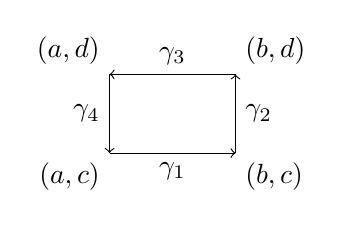
\begin{tikzpicture}
              \draw (0,0) node[below left] {$(a, c)$};
              \draw (0,1) node[above left] {$(a, d)$};
              \draw (1.6,0) node[below right] {$(b, c)$};
              \draw (1.6,1) node[above right] {$(b, d)$};

              \node at (0.8,0) [below] {$\gamma_1$};
              \node at (1.6,0.5) [right] {$\gamma_2$};
              \node at (0.8,1) [above] {$\gamma_3$};
              \node at (0,0.5) [left] {$\gamma_4$};

              \draw[->] (0,0) -- (1.6, 0);
              \draw[->] (1.6,0) -- (1.6, 1);
              \draw[->] (1.6,1) -- (0, 1);
              \draw[->] (0,1) -- (0, 0);
        \end{tikzpicture}\]
        То, что мы увидим сейчас, является первым заходом на \emph{формулу Гаусса --- Остроградского}.
        Функция $h$ непрерывна, и можно записать на неё интеграл Лебега: $\int\limits_{P}h(x, y)\d x \d y$.
        Теперь применяя теорему Фубини, раскладываем интеграл в сумму повторных:
        \multline{\int\limits_{\gamma_3^-}f(\_, d)\d x + \int\limits_{\gamma_1^-}f(\_, c)\d x = \int\limits_{a}^{b}\left[f(x, d) - f(x, c)\right]\d x = \int\limits_{a}^{b}\left(\int\limits_{c}^{d}\der{f}{y}\d y\right)\d x
            =\\= \int\limits_{P}h(x, y)\d x \d y =\\=
            \int\limits_{c}^{d}\left(\int\limits_{a}^{b}\der{g}{x}\d x\right)\d y = \int\limits_{c}^{d}\left[g(b, y) - g(a, y)\right]\d y = \int\limits_{\gamma_2}g(b, \_)\d y + \int\limits_{\gamma_4}g(a, \_)\d y}
        Итого, $\int\limits_{\gamma_3^-}f(\_, d)\d x + \int\limits_{\gamma_1^-}f(\_, c)\d x = \int\limits_{\gamma_2}g(b, \_)\d y + \int\limits_{\gamma_4}g(a, \_)\d y$, откуда действительно $\int\limits_{\gamma}\Phi = 0$.
    \item[$\when$] Теперь приведём альтернативное доказательство индукцией по $n$.

    \underline{База:} Случай $n = 1$ тривиален: теорема Ньютона --- Лейбница говорит, что у непрерывной функции есть первообразная.

    \underline{Переход:} Пусть $n > 1$, и для $n - 1$ теорема доказана.
    Рассмотрим $a \in G$, и возьмём прямоугольный параллелепипед со сторонами, параллельными осям координат $P \ni a$.
        Докажем, что на $P$ у $\Phi$ есть первообразная.

    Построим $g(x_1, \dots, x_n) = \int\limits_{a_1}^{x_1}f_1(t, x_2, \dots, x_n)\d t$. Обозначим $\phi_j \coloneqq \der{g}{x_j}$.
        Заметим, что $\phi_1 = \der{g}{x_1} = f_1$.

    Теперь рассмотрим форму $\Psi(x_1, \dots, x_n) = \phi_1 \d x_1 + \dots + \phi_n \d x_n$.
        Эта форма имеет первообразную $g$ на параллелепипеде $P$.

    Теперь посмотрим на $\Phi - \Psi \eqqcolon h_1 \d x_1 + \dots + h_n \d x_n$.
        По построению $h_1 = 0$.
        По условию накрест взятые частные производные равны и $\Phi$, и они равны и $\Psi$, так как у неё есть первообразная.
    Значит, это же верно и для разности, в частности, $\der{h_i}{x_1} = \der{h_1}{x_i} = 0$.
        Иными словами, $\forall i: h_i$ не зависит от $x_1$.

    А раз так, то на $\Phi - \Psi$ можно смотреть, как на форму $(n-1)$-й переменной, и применить индукционное предположение.

    \note{
        Тут есть некоторый обман: производные $\der{\phi_i}{x_j}$ могут просто не существовать.

        Попробуем обойти его так: пусть $\beta \in C^\infty$, с компактным носителем.
        Выберем аппроксимативную единицу $\beta_t(x) = \frac{1}{t^n}\beta(\frac{x}{t})$.

        Назначим $f_k^{(t)} = f_k * \beta_t$, $f_k^{(t)} \underset{t \to 0}\rightrightarrows f_k$.

        Далее у формы $\Phi^{(t)}$ коэффициенты $h_k^{(t)}$ не зависят от $x_1$. А раз они стремятся к $h_k$, то и они не зависят от $x_1$.
        \comment{
        Это было произнесено устно, я наверняка что-то не так записал.
        }
    }
    }
    }
    \theorem[Коши]{
    Пусть $F$ --- голоморфная функция в открытом множестве $G \subset \C$ Тогда дифференциальная форма $F(z)\d z$ замкнута, то есть $\exists G: G'(z) = F(z)$.
        \note{
        Теорема совсем проста, если заранее предположить, что $F'(z)$ непрерывна (а так в итоге и должно получиться, так как $F$ --- аналитична~(\cref{analytic-is-holomorphic})).
        В таком случае имеется следующее более простое доказательство.
        \provehere{
            % Надо проверить второе уранвение Коши --- Римана: $\forall z \in \C: \der{F}{y}(z) = i \der{F}{x}(z)$ (первое выполнено, так как накрест-взятые частные производные равны).
            $\forall z \in \C: \der{F}{y}(z) = i \der{F}{x}(z)$
        пусть $F(z) = u(x, y) + i v(x, y)$.
        \[\der{u}{y} + \der{v}{y} \underset{?}= i\left(\der{u}{x} + \der{v}{x}\right)\]
        то есть $\der{u}{y} = -\der{v}{x}$ и $\der{v}{y} = \der{u}{x}$.
        \comment{Я вообще не понял, что произошло.}
        }
        }
        Теперь докажем теорему Коши вне предположения непрерывности производной.
    \provehere{
    Докажем от противного: пусть форма $F(z)\d z$ не замкнута, $\exists P_0 \subset G: \alpha = \int\limits_{\partial P_0}F(z)\d z \ne 0$.

    Будем потихонечку делить этот прямоугольник на четыре равные части: пусть $P_0 = Q_1 \cup Q_2 \cup Q_3 \cup Q_4$.
        \[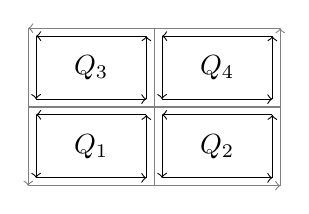
\begin{tikzpicture}
              \draw[->,color=gray] (0,0) -- (3.2, 0);
              \draw[->,color=gray] (3.2,0) -- (3.2, 2);
              \draw[->,color=gray] (3.2,2) -- (0, 2);
              \draw[->,color=gray] (0,2) -- (0, 0);
              \draw[color=gray] (0,1) -- (3.2,1);
              \draw[color=gray] (1.6,0) -- (1.6,2);
              \foreach \x/\y/\i in {0/0/1,1.6/0/2,0/1/3,1.6/1/4} {
                  \draw[->] ({\x+0.1},{\y+0.1}) -- ({\x+1.5}, {\y+0.1});
                  \draw[->] ({\x+1.5},{\y+0.1}) -- ({\x+1.5}, {\y+0.9});
                  \draw[->] ({\x+1.5},{\y+0.9}) -- ({\x+0.1}, {\y+0.9});
                  \draw[->] ({\x+0.1},{\y+0.9}) -- ({\x+0.1}, {\y+0.1});
                  \node at ({\x + 0.8}, {\y + 0.5}) {$Q_{\i}$};
              }
        \end{tikzpicture}\]
    Интеграл по границе по крайней мере одного из $Q_i$ хотя бы $\frac{\alpha}{4}$.
        Назовём этот прямоугольник $P_1$, и продолжим процесс.
        Получим систему вложенных замкнутых прямоугольников $P_0 \supset P_1 \supset \dots$, таких, что $\abs{\int\limits_{\partial P_k}F(z)\d z} \ge \frac{|\alpha|}{4^k}$.
        При этом $l(\partial P_k) = 2^{-k}l(\partial P_0)$, и $\diam (P_k) = 2^{-k} \diam(P_0)$.

    Имеется ровно одна точка $z_0$ в пересечении $\bigcap\limits_{k \ge 0}P_k$.
        Воспользуемся условием того, что $F$ голоморфна в точке $z_0$: $F(z) = F(z_0) + F'(z_0)(z - z_0) + \underbrace{\psi(z)}_{o(|z - z_0|)}$

    Зафиксируем $\eps > 0$. $\exists \delta > 0: |z - z_0| < \delta \then |\psi(z)| \le \eps|z - z_0|$.
        Пусть $k$ настолько велико, что $\diam P_k < \delta$.
    \[\int\limits_{\partial P_k}F(z)\d z = \int\limits_{\partial P_k}[F(z_0) + F'(z_0)(z -z_0)]\d z + \int\limits_{\partial P_k}\psi(z)\d z\]
    Первый интеграл обнуляется, так как это линейная функция по $z$, у неё есть первообразная.
        Оценивая второй интеграл, получаем \[\frac{|\alpha|}{4^k} \le \abs{\int\limits_{\partial P_k}\psi(z)\d z} \le \eps\diam P_k \cdot l(\partial P_0) = 2^{-k}\eps\diam P_0 \cdot 2^{-k}l(\partial P_0) = 4^{-k}\eps \cdot \diam P_0 \cdot l(\partial P_0)\]
    Выбирая довольно маленький $\eps$, получаем, что $|\alpha|$ меньше любого положительного числа.
    }
    }
    \theorem[Об устранимой особенности замкнутой дифференциальной формы]{
        Пускай $\Phi = f \d x + g\d y$ --- непрерывная дифференциальная форма в области $G \subset \C$.

        Если $z_0 \in G$, и $\Phi$ замкнута в $G \sm \{z_0\}$, то $\Phi$ замкнута в $G$.
        \provehere{
            Докажем, что $\forall P \subset G: \int\limits_{\partial P}\Phi = 0$.
            Рассмотрим случаи.
        \bullets{
            \item Если $z_0 \notin P$, то интеграл нуль по условию.
            \item Если $z_0 \in \Int P$, то данный случай сводится к следующему: разобьём прямоугольник на два так, чтобы $z_0$ оказалось на границе:
            \[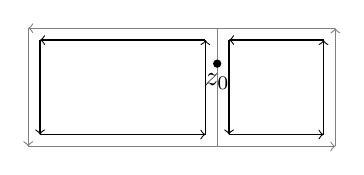
\begin{tikzpicture}[scale=1.5]
                  \draw[->,color=gray] (0,0) -- (2.6, 0);
                  \draw[->,color=gray] (2.6,0) -- (2.6, 1);
                  \draw[->,color=gray] (2.6,1) -- (0, 1);
                  \draw[->,color=gray] (0,1) -- (0, 0);
                  \draw[color=gray] (1.6,0) -- (1.6,1);
                  \fill (1.6,0.7) circle (1pt) node[below] {$z_0$};
                  \foreach \x/\w in {0/1.6, 1.6/1} {
                      \draw[->] ({\x+0.1},{0.1}) -- ({\x+\w-0.1}, {0.1});
                      \draw[->] ({\x+\w-0.1},{0.1}) -- ({\x+\w-0.1}, {0.9});
                      \draw[->] ({\x+\w-0.1},{0.9}) -- ({\x+0.1}, {0.9});
                      \draw[->] ({\x+0.1},{0.9}) -- ({\x+0.1}, {0.1});
                  }
            \end{tikzpicture}\]
            \item Если $z_0 \in \partial P$, то отступим на $\eps$, интеграл по границе $P_\eps$ будет нулём: $\int\limits_{\partial P_\eps}\Phi = 0$.

        Заметим, что $\int\limits_{\partial P_\eps}\Phi \underset{\eps \to 0}\Map \int\limits_{\partial P}\Phi$, так как коэффициенты дифференциальной формы равномерно непрерывны в некоторой окрестности $P$.
            Значит, $\int\limits_{\partial P}\Phi = 0$.
        }
        }
    }
    \theorem[Малая интегральная форма Коши]{
    Пусть $f$ --- голоморфна в области $G$, $B = B(z_0, r)$ --- круг, $\overline{B} \subset G$. Тогда $\forall z \in B$:
    \[f(z) = \frac{1}{2\pi i}\int\limits_{\partial B}\frac{f(\zeta)}{\zeta - z}\d \zeta\]
    \provehere{
    Докажем для некоего фиксированного $z \in B$.

        Рассмотрим функцию $g(\zeta) = \frac{f(z) - f(\zeta)}{z - \zeta}$.
        $g$ голоморфна в области $G \sm \{z\}$. Тем самым, $g(\zeta)\d \zeta$ --- замкнутая форма в $G \sm \{z\}$, а по теореме об устранимой особенности $g(\zeta)\d \zeta$ замкнута в $G$ (доопределим по непрерывности $g(z) \coloneqq f'(z)$).

        Но так как круг --- удобная область, то у $g$ имеется первообразная в некотором круге $B(z_0, r(1 + \eps))$ (где $\eps > 0$ настолько мал, что $B(z_0, r(1 + \eps)) \subset G$),

        Тем самым, $\int\limits_{|z - z_0| = r}\frac{f(z) - f(\zeta)}{z - \zeta}\d \zeta = 0$, откуда \[\int\limits_{|z - z_0| = r}\frac{f(\zeta)}{\zeta - z}\d \zeta = \frac{f(z)}{\zeta - z}\d \zeta = f(z)\int\limits_{|z - z_0| = r}\frac{1}{\zeta - z}\d \zeta = 2\pi i \cdot f(z)\]
    }
    }
    \corollary[Теорема Коши]{
    Если функция голоморфна в области $G \subset \C$, то $\forall z_0 \in G$ функция $f$ раскладывается в некоторый степенной ряд $f(z) = \sum\limits_{n = 0}^{\infty}c_n(z - z_0)^n$, причём радиус сходимости хотя бы $\dist(z_0, \partial G)$.
    \provehere{
        Пусть $r \in (0, \dist(z_0, \partial G))$.
        Рассмотрим $B = B_r(z_0)$. Так как $B \subset G$, то
    \multline{f(z) = \frac{1}{2\pi i}\int\limits_{|z - z_0| = r}\frac{f(\zeta)}{\zeta - z}\d \zeta = \frac{1}{2\pi i}\int\limits_{|z - z_0| = r}\frac{f(\zeta)}{(\zeta - z_0) + (z_0 - z)}\d \zeta =\\= \frac{1}{2\pi i}\int\limits_{|z - z_0| = r}\frac{1}{z - z_0}\cdot \frac{1}{1 - \frac{z - z_0}{\zeta - z_0}}f(\zeta)\d\zeta = \frac{1}{2\pi i}\sum\limits_{j = 0}^{\infty}(z - z_0)^{j + 1}\int\limits_{|z - z_0| = r}\frac{f(\zeta)}{(\zeta - z_0)^{j+1}}\d \zeta}
    Таким образом, мы получили степенной ряд, и так как коэффициенты степенного ряда, раз определены, не зависят от радиуса круга, то радиус сходимости данного ряда хотя бы $\dist(z_0, \partial G)$.
    }
    }
\end{document}
